\section{More discussion on matroid representability}
This chapter will introduce a new concept, a matroid minor, which is crucial when discussing the matroid representability.

In order to introduce a matroid minor, we first need to introduce two operations on matroids: deletion and contraction.

\begin{defn}
Let $M = (E, \mathcal{I})$, $e \in E$ be given.
$M \backslash e$ is defined to be $(E - \{ e \}, \{ I \in \mathcal{I} \mid e \notin I \})$.
\end{defn}

\begin{thm}
Let $M = (E, \mathcal{I})$, $e \in E$ be given.
$M \backslash e$ is indeed a matroid.
\end{thm}

\begin{proof}
Let $M' = M \backslash e = (E', \mathcal{I}')$.
$\emptyset \in \mathcal{I}'$ since $\emptyset \in \mathcal{I}$ and $e \notin \emptyset$.
Let $I \in \mathcal{I}'$ and $J \subseteq I$.
Since $e \notin I$, $e \notin J$.
Since $I \in \mathcal{I}'$, $I \in \mathcal{I}$.
Since $J \subseteq I$, $J \in \mathcal{I}$.
Therefore, $J \in \mathcal{I}'$.
Let $A, B \in \mathcal{I}'$ such that $\lvert A \rvert < \lvert B \rvert$.
Since $A, B \in \mathcal{I}'$, they are in $\mathcal{I}$.
Let $x \in B - A$ such that $A \cup \{ x \} \in \mathcal{I}$.
Since $e \notin B$, $e \neq x$.
Therefore, $e \notin A \cup \{ x \}$.
It means that we have found $x \in B - A$ such that $A \cup \{ x \} \in \mathcal{I}'$.
Since $M'$ satisfies the three properties, it is indeed a matroid.
\end{proof}

The above is the definition of deletion by an element.
It is also possible to define deletion by a subset of $E$.

\begin{defn}
Let $M = (E, \mathcal{I}), X = \{ x_1, \cdots, x_k \} \subseteq E$.
$M \backslash X$ is defined to be $(((M \backslash x_1) \backslash x_2) \cdots) \backslash x_k)$.
\end{defn}

The following theorem shows that the order of deletion does not matter.

\begin{thm}
For any given matroid $M = (E, \mathcal{I})$,
$(M \backslash e) \backslash f = (M \backslash f) \backslash e$ for any $e \neq f \in E$.
\end{thm}

\begin{proof}
First, it is easy to see that $(M \backslash e) \backslash f$ and $(M \backslash f) \backslash e$ have the same ground set, which is $E \backslash \{ e, f \}$.
Therefore, it suffices to check the family of independent sets.
The family of independent sets of $M \backslash e$ is $\mathcal{I}' = \{ I \in \mathcal{I} \mid e \notin I \}$.
The family of independent sets of $(M \backslash e) \backslash f$ is $\mathcal{I}'' = \{ I \in \mathcal{I}' \mid f \notin I \}$.
Obviously, $\mathcal{I}'' \subseteq I$, and, for any $I \in \mathcal{I}$, $I \in \mathcal{I}''$ if and only if $e \notin I$ and $f \notin I$.
Therefore, the family of independent sets of $(M \backslash e) \backslash f = \{ I \in \mathcal{I} \mid \{ e, f \} \cap I = \emptyset \}$.
Now, it is easy to see that $(M \backslash e) \backslash f = (M \backslash f) \backslash e$.
\end{proof}

Here are a few simple yet useful results about deletion.

\begin{thm}
Let a matroid $M = (E, \mathcal{I}), X \subseteq E$ be given.
Let $A$ be an independent set in $M \backslash X$.
Then $A$ is independent in $M$.
\end{thm}

\begin{proof}
A family of independent sets of $M \backslash X$ is $\{ I \in \mathcal{I} \mid (I \cap X) = \emptyset \}$.
It is easy to see that it is a subset of $\mathcal{I}$.
Since $A$ is in the subset of $\mathcal{I}$, $A$ must be in $\mathcal{I}$.
\end{proof}

In other words, this means that deletion never ``adds" a new element to a family of independent sets.

\begin{thm}
The deletion of a loop does not change a family of independent sets.
\end{thm}

\begin{proof}
Let $M = (E, \mathcal{I}), e \in E, \{ e \} \notin \mathcal{I}$.
A family of independent sets of $M \backslash e$ is $\{ I \in \mathcal{I} \mid (I \cap \{ e \}) = \emptyset \}$.
Since $\{ e \}$ is a loop, no independent set can contain $e$.
Therefore, a family of independent sets of $M \backslash e$ is identical to $\mathcal{I}$.
\end{proof}

% \begin{thm}
% Let $M = (E, \mathcal{I})$, $X \subseteq E$ be given.
% $M \backslash X$ is indeed a matroid
% \end{thm}
% 
% \begin{proof}
% Let $M' = (E', \mathcal{I}') = M \backslash X$.
% Since $\emptyset \in \mathcal{I}$ and $X \cap \emptyset = \emptyset$, $\emptyset \in \mathcal{I}'$.
% Let $I \in \mathcal{I}', J \subseteq I$.
% Since $I \in \mathcal{I}$, $J \in \mathcal{I}$.
% Since $J \subseteq I$ and $I \cap X = \emptyset$, $J \cap X = \emptyset$.
% Therefore, $J \in \mathcal{I}'$.
% Let $A, B \in \mathcal{I}'$ such that $\lvert A \rvert < \lvert B \rvert$.
% Since $A, B \in \mathcal{I}'$, we know that $A, B \in \mathcal{I}$.
% Therefore, we can find $x \in B - A$ such that $(A \cup \{ x \}) \in \mathcal{I}$.
% Since $(A \cup \{ x \}) \subseteq (A \cup B)$ and $X \cap A = X \cap B = \emptyset$, $X \cap (A \cup \{ x \}) = \emptyset$.
% Therefore, $A \cup \{ x \} \in \mathcal{I}'$.
% Thus, we have found such $x \in B - A$ that $A \cup \{ x \} \in \mathcal{I}'$.
% Since $M' = M \backslash X$ follows the three properties, it is indeed a matroid. 
% \end{proof}
% 

Since we have defined deletion, we are going to define contraction.
\begin{defn}
Let $M = (E, \mathcal{I})$, $e \in E$ be given.
$M / e$ denotes contraction of $M$ by $e$ and 
$M / e = \begin{cases}
      M \backslash e, \text{if $e$ is a loop},\\
      (E - \{ e \}, \{ I \in \mathcal{I} \mid e \notin I, (I \cup \{ e \}) \in \mathcal{I}\}), \text{ otherwise}.
         \end{cases}$
\end{defn}


\begin{thm}
Contraction by an element indeed generates a matroid.
\end{thm}

\begin{proof}
If $e$ is a loop, $M / e$ is obviously a matroid since we know that deletion always generates a matroid.
Suppose otherwise.
Let $\mathcal{I}'$ denote a family of independent sets of $M / e$.
First, $\emptyset \in \mathcal{I}, e \notin \emptyset$. Since $e$ is not a loop, $(\emptyset \cup \{ e \}) \in \mathcal{I}$.
Therefore, $\emptyset \in \mathcal{I}'$.
Let $I \in \mathcal{I}', J \subseteq I$.
Since $I \in \mathcal{I}$, $J \in \mathcal{I}$.
Since $e \notin I$, $e \notin J$.
Since $(I \cup \{ e \}) \in \mathcal{I}$ and $J \subseteq I$, $(J \cup \{ e \}) \in \mathcal{I}$.
Therefore, $J \in \mathcal{I}'$.
Let $A, B \in \mathcal{I}'$ such that $\lvert A \rvert < \lvert B \rvert$.
Let $A' = A \cup \{ e \}, B' = B \cup \{ e \}$.
Since $A, B \in \mathcal{I}'$, $A', B' \in \mathcal{I}$.
Since $e \notin A, e \notin B$, $\lvert A' \rvert < \lvert B' \rvert$.
Let $x \in B' - A'$ such that $A' \cup \{ x \} \in \mathcal{I}$.
Since $B' - A' = B - A$, $x \in B - A$.
For such $x$, we just showed that $A \cup \{ e \} \cup \{ x \} \in \mathcal{I}$.
Also, $x \neq e$ since $e \in A'$.
Therefore, $A \cup \{ x \} \in \mathcal{I}'$. 
Hence, we have found $x \in B - A$ such that $A \cup \{ x \} \in \mathcal{I}'$.
Since this follows three properties given in the definition, this is indeed a matroid.
Therefore, contraction by an element indeed generates a matroid.
\end{proof}


Now that we have defined contraction of a matroid by an element, we can define contraction by a subset of a ground set.
\begin{defn}
Let $M = (E, \mathcal{I}), X = \{ x_1, \cdots, x_k \} \subseteq E$.
$M / X$ is defined to be $(((M/x_1)/x_2) \cdots)/x_k)$.
\end{defn}

It is not obvious that this is well-defined. 
In other words, it is not obvious that the order of contraction does not matter.
The following theorem shows that the order does not matter.

\begin{thm}
For any given matroid $M = (E, \mathcal{I})$,
$(M / e) / f = (M / f) / e$ for any $e \neq f \in E$.
\end{thm}

\begin{proof}
There are a few cases.
\begin{enumerate}

\item $e, f$ are both loops. \\
$(M / e) / f = (M \backslash e) / f$.
Since deletion of a loop does not change a family of independent sets, $f$ is a loop in $(M \backslash e)$.
Therefore, $(M / e) / f = (M \backslash e) \backslash f$.
Similarly $(M / f) / e = (M \backslash f) / e$.
Since deletion of a loop does not change a family of independent sets, $e$ is a loop in $(M \backslash f)$.
Therefore, $(M / f) / e = (M \backslash f) \backslash e$.
Since the order of deletion does not matter, they are identical.

\item 
One of $e, f$ is a loop, and the other one is not. \\
Without loss of generality, assume $e$ is a loop.
$(M / e) / f = (M \backslash e) / f$.
Since deletion of a loop does not change a family of independent set, a family of independent set of $(M / e)$ is $\mathcal{I}$.
Therefore, a family of independent sets of $(M / e) / f$ is $\mathcal{I}' = \{ I \in \mathcal{I} \mid f \notin I, (I \cup \{ f \}) \in \mathcal{I} \}$.
On the other hand, it is easy to see that $\mathcal{I}'$ is identical to a family of independent sets of $(M / f)$.
Since contraction by an element does not add new elements to a family of independent sets, $e$ is a loop in $(M / f)$.
Since deletion by a loop does not change a family of independent sets, a family of independent sets of $(M / f) / e$ is $\mathcal{I}'$.
Now we confirmed that $(M / e) / f$ and $(M / f) / e$ have the same family of independent sets.
Therefore, $(M / e) / f = (M / f) / e$.

\item Neither of them is a loop, and $\{ e, f \} \in \mathcal{I}$. \\
A family of independent set of $M / e$ is $\mathcal{I}' = \{ I \in \mathcal{I} \mid e \notin I, (I \cup \{ e \}) \in \mathcal{I} \}$.
Since $\{ e, f \} \in \mathcal{I}$, $\{ f \} \in \mathcal{I}'$. 
Therefore, $f$ is not a loop in $M / e$.
Hence, a family of independent sets of $(M / e) / f$ is $\mathcal{I}'' = \{ I \in \mathcal{I}' \mid f \notin I, (I \cup \{ f \}) \in \mathcal{I}' \}$.
$\mathcal{I}''$ is actually equivalent to $S = \{ I \in \mathcal{I} \mid e \notin I, f \notin I, (I \cup \{ e, f \}) \in \mathcal{I} \}$.
We can prove $\mathcal{I}'' = S$ by starting to show that $\mathcal{I}'' \subseteq S$.
Let $I \in \mathcal{I}''$.
Since $I$ is an independent set of $(M / e) / f$, we know that $e, f \notin I$.
Since $(I \cup \{ f \}) \in \mathcal{I}'$, we also know that $((I \cup \{ f \}) \cup \{ e \}) \in \mathcal{I}$.
Therefore, $(I \cup \{ e, f \}) \in \mathcal{I}$.
Thus $I \in S$, and $\mathcal{I}'' \subseteq S$.
Now, we want to show that $S \subseteq \mathcal{I}''$. 
Let $I \in S$. By the definition of $S$, we know that $e, f \notin I$.
Since $(I \cup \{ e, f \}) \in \mathcal{I}$, we know that $(I \cup \{ e \}) \in \mathcal{I}$.
Since $((I \cup \{ f \}) \cup \{ e \}) \in \mathcal{I}$ and $e \notin (I \cup \{ f \})$, we know that $(I \cup \{ f \}) \in \mathcal{I}'$.
Since $f \notin I$ and $(I \cup \{ f \}) \in \mathcal{I}'$, $I \in \mathcal{I}''$.
Hence, $S \subseteq \mathcal{I}''$.

Combining these two results, we know that $S = \mathcal{I}''$.
By the symmetry, $(M / e) / f$ and $(M / f) / e$ have the same family of independent sets.
Therefore $(M / e) / f = (M / f) / e$.

\item Neither of $e, f$ is a loop, but $\{ e, f \} \notin \mathcal{I}$.\\
A family of independent set of $M / e$ is $\mathcal{I}' = \{ I \in \mathcal{I} \mid e \notin I, (I \cup \{ e \}) \in \mathcal{I} \}$.
Since $\{ e, f \} \notin \mathcal{I}$, $f$ is a loop in $M / e$.
Therefore, $(M / e) / f = (M / e) \backslash f$.
Since the deletion of a loop does not change a family of independent sets, a family of independent sets of $(M / e) / f$ is $\mathcal{I}'$.
By applying the same argument, a family of independent set of $(M / f) / e$ is $\mathcal{I}'' = \{ I \in \mathcal{I} \mid f \notin I, (I \cup \{ f \} ) \in \mathcal{I} \}$.
We want to show that $\mathcal{I}'  = \mathcal{I}''$.
By the symmetry, it suffices to show that $\mathcal{I}' \subseteq \mathcal{I}''$.
Let $I \in \mathcal{I}'$.
Since $\{ e, f \}$ is dependent, $f \notin I$. (Otherwise, $I \cup \{ e \}$ would be dependent.)
Since both $(I \cup \{ e \})$ and $\{ f \}$ are independent, we can grow $\{ f \}$ by adding elements from $(I \cup \{ e \})$ until they have the same size.
Since $\{ e, f\}$ is dependent, we never add $e$.
In other words, we add every element from $\mathcal{I}$.
It means that $I \cup \{ f \}$ is independent.
Therefore, $I \in \mathcal{I}''$, and thus $\mathcal{I}' \subseteq \mathcal{I}''$.
By symmetry, $\mathcal{I}'' \subseteq \mathcal{I}'$.
Therefore, $\mathcal{I}' = \mathcal{I}''$.
\end{enumerate}

Therefore, in any case, $(M / e) / f = (M / f) / e$.
\end{proof}


Here is a simple result about contraction.

\begin{thm}
Let a matroid $M = (E, \mathcal{I}), X \subseteq E$ be given.
Let $A$ be an independent set in $M / X$.
Then $A$ is independent in $M$.
\end{thm}

\begin{proof}
A family of independent sets of $M / X$ is clearly a subset of $\mathcal{I}$ from the definition of contraction.
Since $A$ is in the subset of $\mathcal{I}$, $A$ must be in $\mathcal{I}$.
\end{proof}

In other words, this means that contraction never ``adds" a new element to a family of independent sets just like deletion.
%\item Maybe talk about dual matroid
%  \begin{itemize}
%    \item redefine contraction/deletion in terms of dual
%  \end{itemize}

Now that we have defined contraction and deletion, we can define a \textit{minor} of a matroid.

\begin{defn}
A minor of a matroid is a matroid that can be obtained by a sequence of contraction and deletion operations. (possibly no operation)
\end{defn}

Therefore, most matroids have more than one minor.
To define the matroid minor more concisely, we will prove the following theorem.


\begin{thm}
Let a matroid $M = (E, \mathcal{I})$ and $e \neq f \in E$ be given.
Then $(M / e) \backslash f = (M \backslash f) / e$.
\end{thm}

\begin{proof}
There are a few cases.
\begin{enumerate}
\item
Both $e$ and $f$ are loops.
This case is easy to prove since neither contraction nor deletion add any new elements to a family of independent sets.
In other words, $f$ is a loop in $(M / e)$ and $e$ is a loop in $(M \backslash f)$.
$(M / e) \backslash f = (M \backslash e) \backslash f = (M \backslash f) \backslash e = (M \backslash f) / e$
\item
$e$ is a loop, but $f$ is not a loop.
$(M / e) \backslash f = (M \backslash e) \backslash f$ since $e$ is a loop.
$(M \backslash f) / e = (M \backslash f) \backslash e$ since $e$ is a loop in $(M \backslash f)$.
We know that the order of deletion does not matter, so they are equivalent.
\item
$e$ is not a loop, but $f$ is a loop.
Since the deletion of $f$ does not change a family of independent sets,
both $M$ and $(M \backslash f)$ have the same family of independent sets, although their ground sets are not identical.
Therefore, $(M / e)$ and $(M \backslash f) / e$ have the same family of independent sets from the definition of contraction.
Since we know that contraction does not add a new independent set, $f$ is a loop in $(M / e)$.
Therefore, deletion of $f$ does not change the family of independent sets.
Hence, we know that $(M / e) \backslash f$ and $(M \backslash f) / e$ have the same ground set and the same family of independent sets, so they are identical.
\item
Neither $e$ nor $f$ is a loop.
Let $X \subseteq E - \{e, f\}$.
$X$ is independent in $(M / e) \backslash f$ if and only if $X$ is independent in $(M / e)$.
$X$ is independent in $(M / e)$ if and only if $(X \cup \{ e \})$ is independent in $M$.
On the other hand, $X$ is independent in $(M \backslash f) / e$ if and only if $X \cup \{ e \}$ is independent in $(M \backslash f)$.
$X \cup \{ e \}$ is independent in $(M \backslash f)$ if and only if $X \cup \{ e \}$ is independent in $M$.
Therefore, $X$ is independent in $(M / e) \backslash f$ if and only if $X$ is independent in $(M \backslash f) / e$.
Since $(M / e) \backslash f$ and $(M \backslash f) / e$ have the same ground set and the same family of independent sets, they are identical.
\end{enumerate}
Therefore, in every case, $(M / e) \backslash f$ is identical to $(M \backslash f) / e$.
\end{proof}

By this theorem, we know that any series of operations can be expressed as $(M / A) \backslash B$ where $A, B$ are disjoint subsets of $E$.
Therefore, the following definition is equivalent to the previous definition.

\begin{defn}
Let $M = (E, \mathcal{I})$ be given.
Let $A, B$ be disjoint subsets of $E$.
Then a matroid $(M / A) \backslash B$ is called a minor of $M$.
\end{defn}

Moreover, if $A \cup B \neq \emptyset$, we call $(M / A) \backslash B$ a \textit{proper minor}.

Of course, we could have defined a minor as $(M \backslash A) / B$ instead of $(M / A) \backslash B$.


\subsection{What do contraction and deletion mean in graphs and vector spaces?}
Deletion of a vector in the vector space is simply removing such a vector from the set.
Contraction, however, is more complicated.
In vector spaces, contraction can be considered as projection to its orthogonal vector as showin in the figure 2.
In graphs, deletion of an edge simply removes an edge. Contraction of an edge combines the two nodes that the edge connects as shown in the figure 3.

\begin{figure}
  \centering
    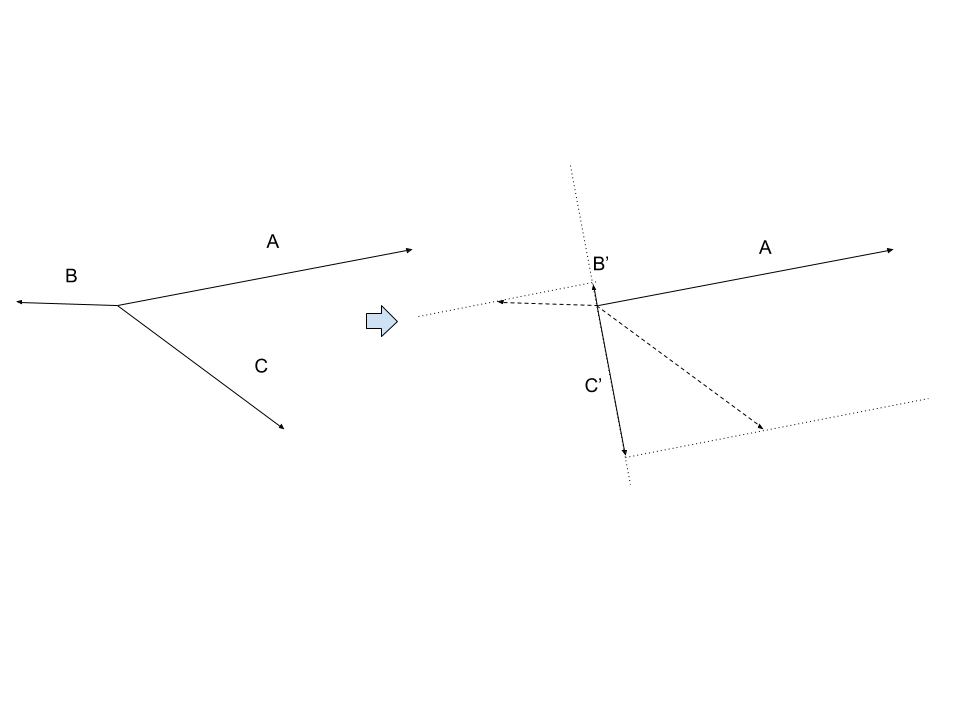
\includegraphics[width=0.8\textwidth,natwidth=610,natheight=642]{vectors.png}
    \caption{Contraction by a vector A}
  \label{fig:test}
\end{figure}

\begin{figure}
  \centering
    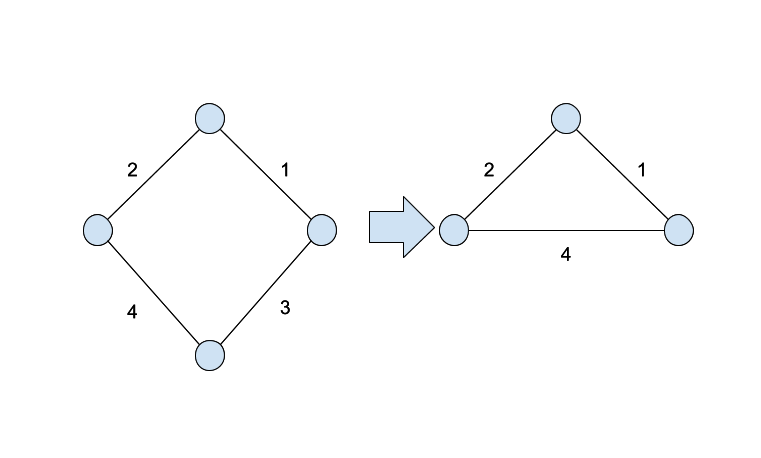
\includegraphics[width=0.8\textwidth,natwidth=610,natheight=642]{graphs.png}
    \caption{Contraction by an edge 3}
  \label{fig:test}
\end{figure}



\subsection{Why do these matter?}
The discussion of contraction and deletion is very important when discussing the representability of matroids since if a matroid is representable over some field $\mathbb{F}$, its minor is always representable over $\mathbb{F}$.

\begin{thm}
Let a matroid $M = (E, \mathcal{I})$ such that it is representable over $\mathbb{F}$.
Any minor of $M$ is representable over $\mathbb{F}$.
\end{thm}

\begin{proof}
It suffices to show that $M / e$ and $M \backslash e$ are both representable over $\mathbb{F}$ for any $e \in E$.
Let $r$ be a rank of $M$, $n = \lvert E \rvert$.
Let $e \in E$ be given.
Without loss of generality, we can assume $E = \{ 1, 2, \cdots, n \}$ and $e = n$.
Let $A = \begin{pmatrix}u_1 u_2 \cdots u_n\end{pmatrix} \in \mathbb{F}^{r \times n}$ be a matrix such that the column matroid of $M$ is identical to $A$.
(We can find such a matrix since we can find a matrix whose column matroid is isomorphic and we can simply permute the column vectors in it)

\begin{enumerate}
\item 
  First, we prove the case of deletion.
  We claim that $M \backslash e$ is isomorphic to the column matroid of $\begin{pmatrix} u_1 u_2 \cdots u_{n-1} \end{pmatrix}$.
  We prove so by comparing the independent sets of each matroid.
  By definition, $M \backslash e = (E - \{ e \}, \{ I \in \mathcal{I} \mid e \notin I \})$.
  Let $U = \{ u_{i_1}, u_{i_2}, \cdots, u_{i_k} \}$ be a subset of $\{ u_1, u_2, \cdots, u_{n-1} \}$.
  We want to show that $U$ is linearly independent if and only if $\{ i_1, i_2, \cdots, i_k \}$ is independent in $M \backslash e$.
  Suppose $U$ is linearly independent. 
  Then $\{ i_1, i_2, \cdots, i_k \}$ is independent in the column matroid of $A$.
  Since $\{ i_1, i_2, \cdots, i_k \}$ is in $\mathcal{I}$ and does not contain $e = n$, it is independent in $M \backslash e$ as well.
  Suppose $U$ is linearly dependent. 
  Then $\{ i_1, i_2, \cdots, i_k \}$ is dependent in the column matroid of $A$.
  Since $\{ i_1, i_2, \cdots, i_k \}$ is not in $\mathcal{I}$, it is dependent in $M \backslash e$ as well.
  Therefore, $M \backslash e$ is representable over $\mathbb{F}$.
\item
  Next, we prove the case of contraction.
  First, assume $e$ is a loop.
  In this case, $M / e = M \backslash e$ by definition.
  We proved above that $M \backslash e$ is representable over $\mathbb{F}$.
  Now, assume that $e$ is not a loop.
  Then the corresponding column of $A$ must not be a zero vector.
  We claim that $M / e$ is identical to the column matroid of $B \in \mathbb{F}^{r \times (n-1)}$, 
  where $i$th column of $B$, $b_i$, is $\displaystyle u_i - \frac{u_i \cdot u_n}{u_n \cdot u_n} u_n$.
  (This makes sense since we are assuming that $u_n$ is not a zero vector.)
  We prove the proposition by comparing the independent sets of each matroid.
  By definition, $M / e = (E - \{ e \}, \{ I \in \mathcal{I} \mid e \notin I, (e \cup I) \in \mathcal{I}\})$.
  Let $X = \{ i_1, i_2, \cdots, i_k \} \subseteq E - \{ n \}$ be given. \\
  $X$ is independent in $M / e$ \\
  $\iff$ $X \cup \{ n \}$ is independent in $M$ \\
  $\iff$ $\{ i_1, i_2, \cdots, i_k, n \}$ is independent in $M$ \\
  $\iff$ $U = \{ u_{i_1}, u_{i_2}, \cdots, u_{i_k}, u_{n} \}$ is linearly independent \\
  We are going to take a close look at this set of vectors.
  Suppose $U$ is linearly independent.
  We want to show that a set of corresponding column vectors of $B$ is linearly independent.
  Let $c_1, c_2, \cdots, c_k \in \mathbb{F}$ be given such that $c_1 b_{i_1} + \cdots + c_k b_{i_k} = 0$.\\
  \begin{align*}\displaystyle 
  0 &= c_1 b_{i_1} + \cdots + c_k b_{i_k}  \\
    &= c_1 u_{i_1} + \cdots + c_k u_{i_k} - \Big( \sum_{j = 1}^{k} c_j \frac{u_{i_j} \cdot u_n}{u_n \cdot u_n} \Big) u_n
  \end{align*}
  Since $U$ is linearly independent, $c_1, \cdots, c_k$ must be all 0.
  Therefore, a set of corresponding column vectors of $B$ is linearly independent.
  Now, suppose a set of corresponding column vectors of $B$ is linearly independent.
  We want to show that $U$ is linearly independent.
  Let $c_1, c_2, \cdots, c_k, c \in \mathbb{F}$ be given such that $c_1 u_{i_1} + \cdots + c_k u_{i_k} + c u_n = 0$.\\
  \begin{align*}\displaystyle
  c_1 b_{i_1} + \cdots + c_k b_{i_k}
%  &= \sum_{j=1,\cdots,k} c_j b_{i_j}  \\
  &= c_1 u_{i_1} + c_2 u_{i_2} + \cdots + c_k u_{i_k} - \sum_{j=1,\cdots,k} c_j \frac{u_{i_j} \cdot u_n}{u_n \cdot u_n} u_n  \\
  &= -c u_n - \sum_{j=1,\cdots,k} c_j \frac{u_{i_j} \cdot u_n}{u_n \cdot u_n} u_n \\
  &= -\Big(c + \sum_{j=1,\cdots,k} c_j \frac{u_{i_j} \cdot u_n}{u_n \cdot u_n}\Big)u_n \\
  &= -\frac{\Big(c({u_n \cdot u_n}) + \sum_{j=1,\cdots,k} c_j (u_{i_j} \cdot u_n)\Big)}{u_n \cdot u_n}u_n \\
  &= -\frac{(c_1 u_{i_1} + c_2 u_{i_2} + \cdots + c_k u_{i_k} + c u_n) \cdot u_n}{u_n \cdot u_n}u_n \\
  &= 0.\end{align*}
  Therefore, $c_1, c_2, \cdots, c_k$ are all 0.
  Since $u_n$ is nonzero and $c u_n = 0$, we know that $c$ is 0 as well.
  Therefore, we know that $U$ is linearly independent.
  Now we have proved that $\{ u_{i_1}, u_{i_2}, \cdots, u_{i_k}, u_{n} \}$ is linearly independent 
  if and only if $\{ b_{i_1}, b_{i_2}, \cdots, b_{i_k} \}$ is linearly independent.
  $\{ b_{i_1}, b_{i_2}, \cdots, b_{i_k} \}$ is linearly independent if and only if $\{ i_1, i_2, \cdots, i_k \}$ is independent in the column matroid of $B$. 
  In conclusion, a subset of $E - \{ e \}$, $X = \{ i_1, i_2, \cdots, i_k \}$, is independent in $M / e$ if and only if $X$ is independent in the column matroid of $B$.
  Therefore, the column matroid of $B$ is identical to $M / e$ since they have the same family of independent sets.
\end{enumerate}
Hence, we have proved that any minor of $M$ is always representable.
\end{proof}

However, neither the converse nor the inverse of this theorem is always true.
Any matroid has a representable minor since we can get a representable minor by deleting elements so that the ground set has at most 3 elements.
Also, $U_{2, 4}$ is not a binary matroid, but any minor of it only contains at most 3 elements, so we know that any minor of $U_{2,4}$ is regular by the theorem.
Rota's conjecture is about unrepresentable matroids any of whose minor is representable.
It will be discussed in the next chapter.


